\documentclass[a4paper,10pt]{article}
\usepackage[utf8]{inputenc}

% increase margins
\usepackage{fullpage}
\usepackage[left=1in,top=1in,right=1in,bottom=1in,headheight=3ex,headsep=3ex]{geometry}

% this puts two lines between paragraphs and no indent
\usepackage[parfill]{parskip}

% set up colors
\usepackage{array, xcolor}
\usepackage{color,hyperref}
\usepackage{graphicx}

\definecolor{torontoblue}{HTML}{00204E}
\definecolor{linkblue}{HTML}{0000FF}

% define hyperlink style
\hypersetup{colorlinks,breaklinks,
            linkcolor=linkblue,urlcolor=linkblue,
            anchorcolor=linkblue,citecolor=linkblue}

%opening
\title{Weekly Journal}
\author{Leila Uy}



\begin{document}

\maketitle

%this is commented out, no need for abstract in  your weekly assignment
% \begin{abstract}
% 
% \end{abstract}

\section{Work Update}

This past week, I focused mainly on reading the assigned material and practicing parallel programming in R. The week was busy with personal 
matters like my friend's wedding and holidays so I was not able to read up on GRASS or thoroughly read the code base as much I hoped to.

\subsection{Parallel programming}

\subsubsection{My Computer Specs and AWS}
The first function that any parallel R tutorial tells you to call is \verb|detectCores(logical = True)| and \verb|detectCores(logical = False)|.
This function returns the number of available hardware threads and cores. For my computer, I have 4 threads and 2 processors. Since I have only 
2 cores, I have been very careful on trying small parallel programming tasks on my laptop, but Jishnu and I started discussions on possibilities 
for small-scale testing to avoid unneccessary AWS charges. We are hoping to test future code on his computer with smaller data sets before 
moving to AWS. This would include experimenting with parsec (access via cloud), live coding, or constant communication of GitHub updates 
(pull requests). 

\subsubsection{R}
I went through \textbf{many} resources for parallel R. Some resources were good \cite{gera2020, hallquist2018, martius2020, tinakarimi2020} 
and some were bad. One of the main things that I discovered is that parallel R will work differently depending on the OS of your computer. For example, I was encountering problems with some functions 
in the R parallel package in Windows. The function \verb|mclapply| will not work in parallel because of how workers are managed. In addition, 
a socket cluster and fork cluster are different and forking will only work in a Unix-like system \cite{hallquist2018}.

\subsubsection{Code Base and Amdahl's Law}
I looked at the code base to get an idea of what it is trying to achieve and the steps it takes to achieve it, but one of the things I 
want to do with the code base in the future is go line-by-line in-depth. From there, I want to create a simple flowchart of the code and 
find the best place to preform parallelism.
\begin{figure}[h!]
    \caption{Example of a flowchart of a simple parallel process \cite{gera2020}}
    \centering
    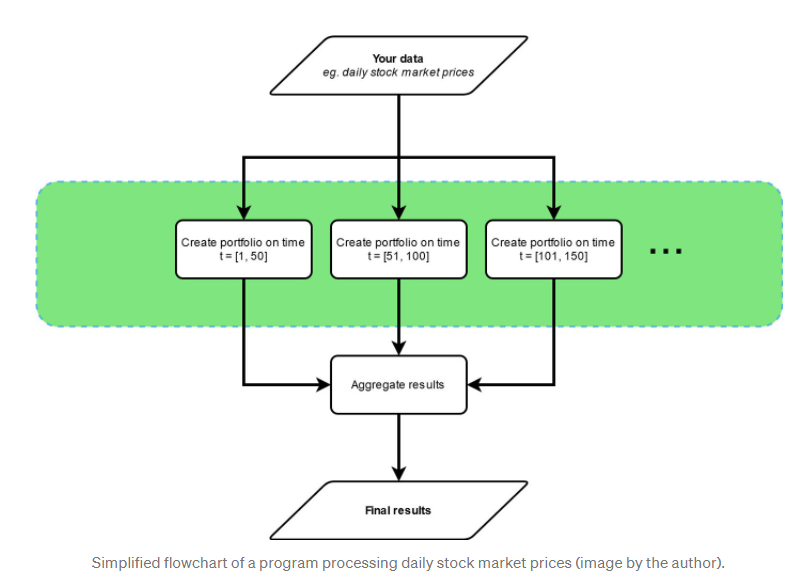
\includegraphics[scale=0.3]{flowchart.png}
\end{figure}

Also, I read about Amdahl's Law which is often used in parallel computing to predict theoretical speedup with multiple processors. \cite{hallquist2018}
I really want to try predicting the speedup of the parallelization then time the process to see if the prediction was close.

\subsection{Future Tasks}
This is what I am hoping to do next.
\begin{itemize}
    \item Comment through the code base
    \item Experiment with parallel GRASS + R
    \item Set up a code sharing process for small scale testing
    \item Create a flow chart for a parallel version of the code base
    \item Time the serial version of the code base with small data sets and calculate Amdahl's Law
\end{itemize}

\section{Literature Review}
The IPCC has many useful reports and resources that will be useful in the future like the "Climate Change and Land" special report for August 2019. 
The assigned reading this week focused on greenhouse gas (GHG) scenerios ("alternative images of how the future might unfold" \cite{ipcc2000}). 
They determined that there are 4 mains storylines (A1, A2, B1, B2) with 40 resulting scenerios. These scenerios were derived from several factors including 
the 3 main driving forces: population prediction, economic development, and structural and technological change.

After reading the article, I had an idea that requires further discussion. It would be interesting to create interpolated GHG emission maps along with 
our ecoregion maps to find patterns or spatial auto-correlation between the anthropo-scene and emissions.
    

% this info creates the bibliography
% YOU WILL NEED TO CHANGE THIS PATH TO THE LOCATION OF THE BIB file
\bibliography{./agclimate.bib}
\bibliographystyle{plain}


\end{document}
